\documentclass[tikz]{standalone}

\usepackage{ctex}

\usepackage{bm}

\usepackage{tikz}

\tikzset{>=latex}

\newcommand{\xOy}[4]{
	\draw[thick, <->](0, #4)node[left]{$#3$}--(0, 0)node[shift={(-135:7pt)}]{$O$}--(#2, 0)node[right]{$#1$}
}

\usetikzlibrary{circuits.ee.IEC}
\usetikzlibrary{angles, quotes}

\usepackage{siunitx}
\sisetup{separate-uncertainty = true}

\newcommand{\nucli}[2]{{^{#1}\mathrm{#2}}}
\newcommand{\nuc}[1]{\mathrm{#1}}

\newcommand*{\CM}{_{\mathrm C}}
\newcommand*{\LAB}{_{\mathrm L}}
\newcommand*{\sca}{{\mathrm{sc}}}

\begin{document}

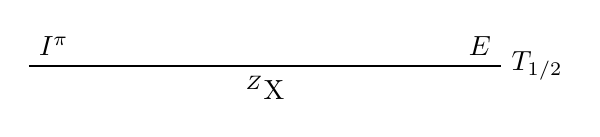
\begin{tikzpicture}
	\draw[thick](0, 0)node[above right]{$I^\pi$}--(6, 0)node[midway, below]{$\nucli ZX$}node[above left]{$E$}node[right]{$T_{1/2}$};
\end{tikzpicture}

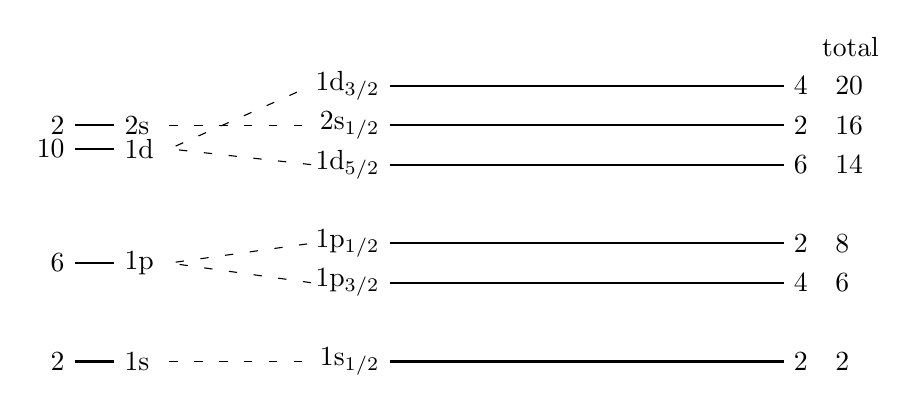
\begin{tikzpicture}
	% 1s
	\draw[thick](-4, 0)node[left]{2}--(-3.5, 0)node[right]{1s};
	\draw[loosely dashed](-2.8, 0)--(-1, 0);
	\draw[thick](0, 0)node[left]{1s$_{1/2}$}--(5, 0)node[right]{2\quad 2};
	% 1p
	\draw[thick](-4, 1.25)node[left]{6}--(-3.5, 1.25)node[right]{1p};
	\draw[loosely dashed](-1, 1)--(-2.8, 1.25)--(-1, 1.5);
	\draw[thick](0, 1)node[left]{1p$_{3/2}$}--(5, 1)node[right]{4\quad 6};
	\draw[thick](0, 1.5)node[left]{1p$_{1/2}$}--(5, 1.5)node[right]{2\quad 8};
	% 1d
	\draw[thick](-4, 2.7)node[left]{10}--(-3.5, 2.7)node[right]{1d};
	\draw[loosely dashed](-1, 2.5)--(-2.8, 2.7)--(-1, 3.5);
	\draw[thick](0, 2.5)node[left]{1d$_{5/2}$}--(5, 2.5)node[right]{6\quad 14};
	\draw[thick](0, 3.5)node[left]{1d$_{3/2}$}--(5, 3.5)node[right]{4\quad 20};
	% 2s
	\draw[thick](-4, 3)node[left]{2}--(-3.5, 3)node[right]{2s};
	\draw[loosely dashed](-2.8, 3)--(-1, 3);
	\draw[thick](0, 3)node[left]{2s$_{1/2}$}--(5, 3)node[right]{2\quad 16};
    \node at (6-0.15, 4) {total};
\end{tikzpicture}

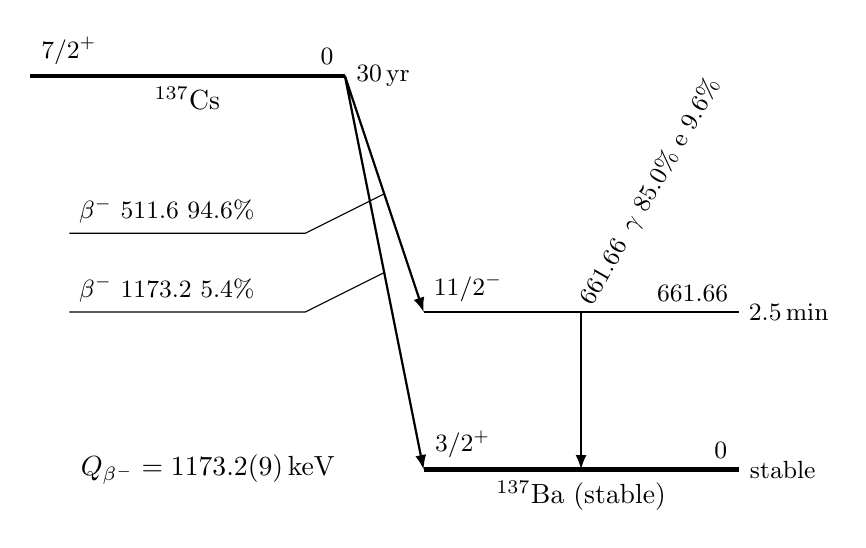
\begin{tikzpicture}
    \draw[ultra thick](-4, 5)node[above right]{\small$7/2^+$}--(0, 5)node[midway, below]{$\nucli{137}{Cs}$}node[above left]{\small 0}node[right]{\small\SI{30}{yr}};
    \draw[thick, latex-latex](1, 2)--(0, 5)--(1, 0);%node[midway, right]{94.4\%}node[midway, left]{5.6\%};
    \draw(.5, 3.5)--(-.5, 3)--(-3.5, 3)node[above right]{\small$\beta^-$ 511.6 94.6\%};
    \draw(.5, 2.5)--(-.5, 2)--(-3.5, 2)node[above right]{\small$\beta^-$ 1173.2 5.4\%};
    \draw[thick](1, 2)node[above right]{\small$11/2^-$}--(5, 2)node[above left]{\small 661.66}node[right]{\small$\SI{2.5}{min}$};
    \draw[ultra thick](1, 0)node[above right]{\small$3/2^+$}--(5, 0)node[midway, below]{$\nucli{137}{Ba}$ (stable)}node[above left]{\small 0}node[right]{\small stable};
    \draw[thick, latex-](3, 0)--(3, 2)node[right, rotate=60]{\small 661.66\enspace$\gamma$ 85.0\% e 9.6\%};%node[midway, right]{\small 661.66};
    \node[left]{$Q_{\beta^-}=\SI{1173.2+-0.9}{keV}$};
\end{tikzpicture}

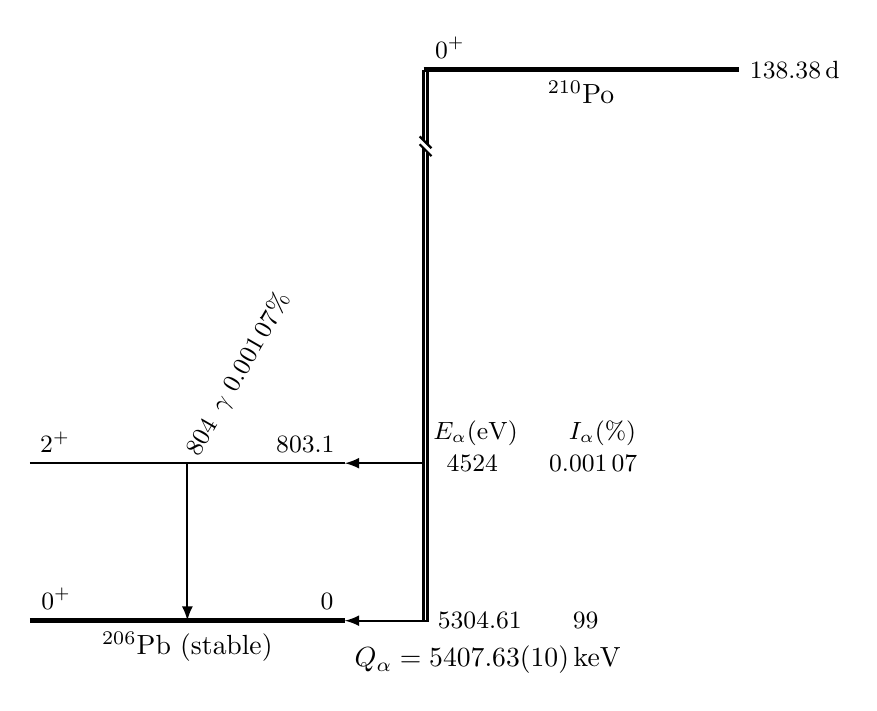
\begin{tikzpicture}
    \node[right]at(4, -.5){$Q_\alpha=\SI{5407.63+-0.10}{keV}$};
    \draw[ultra thick](0, 0)node[above right]{\small $0^+$}--(4, 0)node[midway, below]{$\nucli{206}{Pb}$ (stable)}node[above left]{\small 0};
    \draw[thick](0, 2)node[above right]{\small $2^+$}--(4, 2)node[above left]{\small 803.1};
    \draw[thick, latex-](2, 0)--(2, 2)node[right, rotate=60]{\small 804\enspace$\gamma$ \num{0.00107}\%};
    \draw[thick, latex-](4, 2)--(5, 2)node[right]{\small\enspace\num{4524}\qquad\num{0.00107}};
    \node[above right]at(5, 2.1){\small$E_\alpha(\si{eV})\qquad I_\alpha(\%)$};
    \draw[thick](5, 0)--(5, 6);
    \draw[thick, latex-](4, 0)--(5.05, 0)node[right]{\small\num{5304.61}\qquad 99}--(5.05, 5.95);
    \draw[thick](4.95, 6.05)--(5.1, 5.9);
    \draw[thick](4.95, 6.15)--(5.1, 6);
    \draw[thick](5, 6.1)--(5, 7);
    \draw[thick](5.05, 6.05)--(5.05, 7);
    \draw[ultra thick](5, 7)node[above right]{\small $0^+$}--(9, 7)node[midway, below]{$\nucli{210}{Po}$}node[right]{\small\SI{138.38}{d}};
\end{tikzpicture}

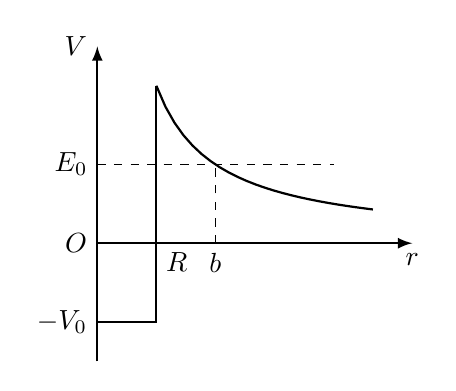
\begin{tikzpicture}
    \draw[thick, -latex](0, -1.5)--(0, 2.5)node[left]{$V$};
    \draw[thick, -latex](0, 0)node[left]{$O$}--(4, 0)node[below]{$r$};
    \draw[dashed](0, 1)node[left]{$E_0$}--(3, 1);
    \draw[thick](0, -1)node[left]{$-V_0$}--(.75, -1)--(.75, 2);
    \draw[dashed](1.5, 0)node[below]{$b$}--(1.5, 1);
    \node[below right]at(.75, 0){$R$};
    \draw[thick, domain=.75:3.5]plot(\x, {1.5/\x});
\end{tikzpicture}

\begin{tikzpicture}
    \draw[ultra thick](0, 4)node[above right]{\small$1^+$}--(4, 4)node[midway, below]{$\nucli{64}{Cu}$}node[right]{\small\SI{12.70}{h}};
    \draw[ultra thick](-4, 0)node[above right]{\small$0^+$}--(-1, 0)node[midway, below]{$\nucli{64}{Ni}$(稳定)}node[above left]{\small0};
    \draw[thick](-4, 3)node[above right]{$2^+$}--(-1, 3)node[above left]{\small\num{1345.8}};
    \draw[ultra thick](5, 2.5)node[above right]{\small$0^+$}--(7, 2.5)node[midway, below]{$\nucli{64}{Zn}$(稳定)};
    \draw[thick, -latex](4, 4)--(5, 2.5);
    \draw[thick, -latex](0, 4)--(-1, 3);
    \draw[thick, -latex](0, 4)--(-1, 0);
    \draw[thick, -latex](0, 4)--(0, 2)--(-1, 0);
    \draw[thick, latex-](-2.8, 0)--(-2.8, 3)node[right, rotate=60]{\small\num{1345.77}\enspace$\gamma$ \num{0.48}\%};
    \draw(4.5, 3.25)--(4, 2.8)--(.5, 2.8)node[above right]{\small$\beta^-$\enspace\SI{578.2}{keV} 37.1\%}node[below right]{\small $Q_{\beta^-}=\SI{578.2+-1.5}{keV}$};
    \draw(-.5, 3.5)--(.5, 1.65)node[above right]{\small EC$_1$}--(4, 1.65)node[above left]{\small 0.48\%};
    \draw(-.5, 2)--(.5, 1)node[above right]{\small EC$_2$}--(4, 1)node[above left]{\small 44.5\%};
    \draw(-.5, 1)--(.5, .35)node[above right]{\small$\beta^+$\enspace\SI{652.9}{keV}\enspace\,17.9\%}node[below right]{\small$Q_{\mathrm{EC}}=\SI{1674.9+-0.8}{keV}$}--(4, .35);
\end{tikzpicture}

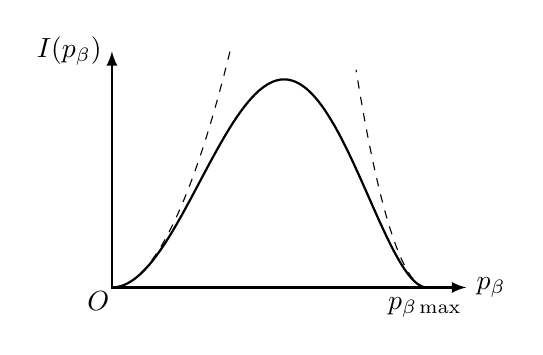
\begin{tikzpicture}
    \xOy{p_\beta}{4.5}{I(p_\beta)}{3};
    \draw[thick, domain=0:4, samples=100]plot(\x, {(2-sqrt(\x^2+9)+3)^2*\x^2/3})node[below]{$p_{\beta\max{}}$};
    \draw[dashed](0, 0)parabola(1.5, 3);
    \draw[dashed](4, 0)parabola(3.1, 2.7648);
\end{tikzpicture}

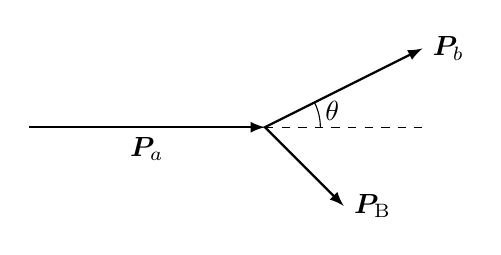
\begin{tikzpicture}
    \coordinate(o)at(0, 0);
    \coordinate(b)at(2, 1);
    \coordinate(c)at(2, 0);
    \coordinate(B)at(1, -1);
    \draw[thick, -latex](-3, 0)--(o)node[midway, below]{$\bm P_a$};
    \draw[thick, latex-latex](B)node[right]{$\bm P_{\nuc B}$}--(o)--(b)node[right]{$\bm P_b$};
    \draw[dashed](o)--(c);
    \pic["$\theta$", draw, angle eccentricity=1.25, angle radius=20]{angle=c--o--b};
\end{tikzpicture}

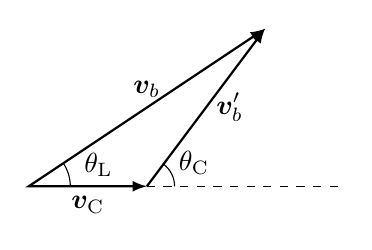
\begin{tikzpicture}
    \coordinate(A)at(0, 0);
    \coordinate(C)at(1.5, 0);
    \coordinate(b)at(3, 2);
    \coordinate(f)at(4, 0);
    % \coordinate(a)at(-1, 0);
    \draw[dashed](C)--(f);
    \draw[thick, -latex](C)--(b)node[midway, right]{$\bm v_b'$};
    \draw[thick, latex-latex](C)--(A)node[midway, below]{$\bm v\CM$}--(b)node[midway, above]{$\bm v_b$};
    \pic["$\theta\LAB$", draw, angle eccentricity=1.75, angle radius=15]{angle=f--A--b};
    \pic["$\theta\CM$", draw, angle eccentricity=1.9, angle radius=10]{angle=f--C--b};
\end{tikzpicture}

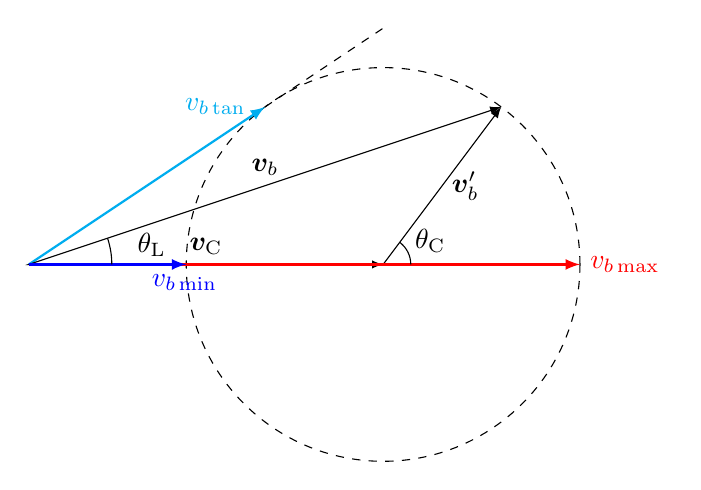
\begin{tikzpicture}
    \coordinate(A)at(-3, 0);
    \coordinate(C)at(1.5, 0);
    \coordinate(b)at(3, 2);
    \coordinate(f)at(4, 0);
    \coordinate(a)at(-1, 0);
    \coordinate(t)at(0, 2);
    \draw[dashed](C)circle(2.5);
    \draw[dashed](t)--(1.5, 3);
    \draw[cyan, thick, -latex](A)--(t)node[left]{$v_{b\tan}~$};
    \draw[-latex](C)--(b)node[midway, right]{$\bm v_b'$};
    \draw[latex-latex](C)--(A)node[midway, above]{$\bm v\CM$}--(b)node[midway, above]{$\bm v_b$};
    \draw[red, thick, -latex](A)--(f)node[right]{$v_{b\max{}}$};
    \draw[blue, thick, -latex](A)--(a)node[below]{$v_{b\min{}}$};
    \pic["$\theta\LAB$", draw, angle eccentricity=1.5, angle radius=30]{angle=f--A--b};
    \pic["$\theta\CM$", draw, angle eccentricity=1.9, angle radius=10]{angle=f--C--b};
\end{tikzpicture}

\begin{tikzpicture}
    \coordinate(o)at(0, 0);
    \coordinate(C)at(1.5, 0);
    \coordinate(b)at(3, 2);
    \coordinate(a)at(4, 0);
    \coordinate(d)at(-1, 0);
    \draw[dashed](C)circle(2.5);
    \draw[-latex](C)--(b)node[midway, right]{$\bm v_b'$};
    \draw[latex-latex](C)--(o)node[midway, below]{$\bm v\CM$}--(b)node[midway, above]{$\bm v_b$};
    \draw[red, thick, -latex](o)--(a)node[right]{$v_{b\max{}}$};
    \draw[blue, thick, -latex](o)--(d)node[left]{$v_{b\min{}}$};
    \pic["$\theta\LAB$", draw, angle eccentricity=1.75, angle radius=15]{angle=a--o--b};
    \pic["$\theta\CM$", draw, angle eccentricity=1.9, angle radius=10]{angle=a--C--b};
\end{tikzpicture}

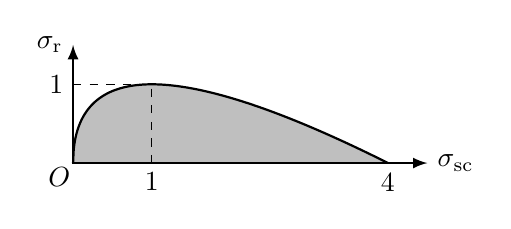
\begin{tikzpicture}
    \draw[thick, domain=0:4, samples=500, fill=gray!50]plot(\x, {2*sqrt(\x)-\x})node[below]{4};
    \xOy{\sigma_\sca}{4.5}{\sigma_\mathrm r}{1.5};
    \draw[dashed](0, 1)node[left]{1}--(1, 1)--(1, 0)node[below]{1};
\end{tikzpicture}

\begin{tikzpicture}
    \node at(0, 5){直接致电离辐射};
    \node at(7, 5){间接致电离辐射};
    \node(e)at(0,4){快电子};
    \node(X)at(7,4){电磁辐射X,$\gamma$};
    \node(C)at(0,0){重带电粒子};
    \node(n)at(7,0){中子};
    \draw[thick,-latex](X)--(e)node[midway,above]{次级电子}node[midway, below]{光原子反应};
    \draw[thick, -latex](n)--(X)node[midway, right]{原子核(n,$\gamma$)};
    \draw[thick, -latex](n)--(C)node[midway,above]{次级重带电粒子}node[midway, below]{核反应(n,c) (n,f)};
    \draw[thick, -latex](n)--(e)node[midway, sloped, above]{核反应之后的内转换电子};
\end{tikzpicture}

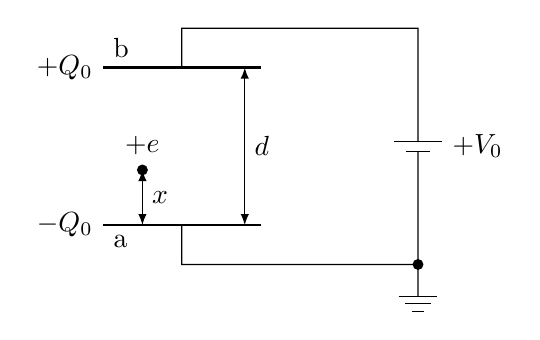
\begin{tikzpicture}[circuit ee IEC]
    \draw [thick] (-4, 2.5) node [left] {$+Q_0$} node [above right] {b} -- (-2, 2.5);
    \draw [thick] (-4, .5) node [left] {$-Q_0$} node [below right] {a} -- (-2, .5);
    \draw [latex-latex] (-2.2, .5) -- (-2.2, 2.5) node [midway, right] {$d$};
    \draw [latex-latex] (-3.5, .5) -- (-3.5, 1.2) node [midway, right] {$x$} node [contact={info={$+e$}}] {};
    \draw (-3, .5) to (-3, 0) to (0, 0) to [ground={at end}] (0, -.5);
    \draw (-3, 2.5) to (-3, 3) to (0, 3) to [battery={info={$+V_0$}}] (0, 0) node [contact] {};
\end{tikzpicture}

\begin{tikzpicture}[circuit ee IEC]
    \draw (6, 0) to (0, 0) to [ground={at end}] (0, -.5);
    \draw (2, 3) to (0, 3) to [battery] (0, 0) node [contact] {};
    \draw (2, 0) node [contact] {} to [resistor={info={$R_L$}}] (2, 1.5) to [capacitor={info={$C_1$}}] (2, 3);
    \draw (3.5, 0) node [contact] {} to [capacitor={info={$C'$}}] (3.5, 1.5) node [contact] {};
    \draw (5, 0) node [contact] {} to [resistor={info={$R_i$}}] (5, 1.5) node [contact] {};
    \draw (6, 0) to [capacitor={info={$C_i$}}] (6, 1.5) to (2, 1.5) node [contact] {};
    \draw [dashed] (4.2, -.2) rectangle (6.5, 1.7);
    \node [above] at (5.25, 1.7) {测量仪器};
    \node [right, align=left] at (7, 1.5) {\small$C_1$探测器电容\\$R_L$负载电阻\\$C'$电缆电容等\\$R_i$测量仪器输入电阻\\$C_i$测量仪器输入电容};
\end{tikzpicture}

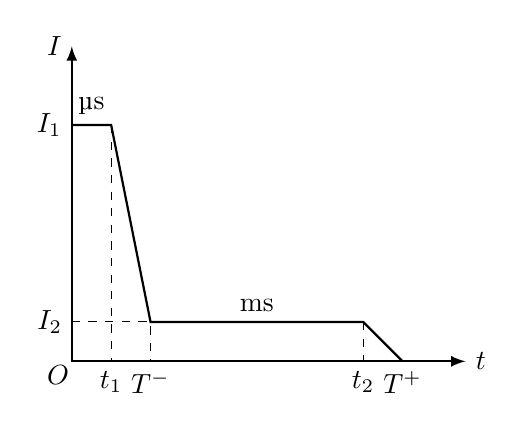
\begin{tikzpicture}
    \xOy t5I4;
    \draw[thick](0, 3)node[left]{$I_1$}--(.5, 3)node[midway, above]{\si{\micro s}}--(1, .5)--(3.7, .5)node[midway, above]{ms}--(4.2, 0)node[below]{$T^+$};
    \draw[dashed](.5, 3)--(.5, 0)node[below]{$t_1$};
    \draw[dashed](0, .5)node[left]{$I_2$}--(1, .5)--(1, 0)node[below]{$T^-$};
    \draw[dashed](3.7, .5)--(3.7, 0)node[below]{$t_2$};
\end{tikzpicture}

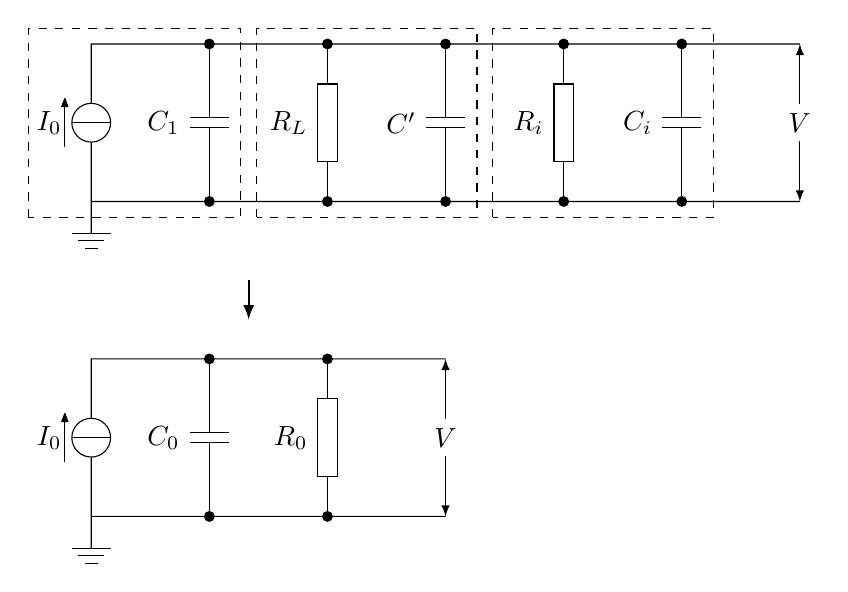
\begin{tikzpicture}[circuit ee IEC]
    \foreach \contact/\x in {1/1.5, 2/3, 3/4.5, 4/6, 5/7.5} {
        \node [contact] (up \contact) at (\x, 2) {};
        \node [contact] (dn \contact) at (\x, 0) {};
    }
    \draw (0, 0) to [current source={direction info={}, info={$I_0$}}] (0, 2) to (9, 2);
    \draw (9, 0) to (0, 0) to [ground={at end}] (0, -.5);
    \draw (dn 1) to [capacitor={info={$C_1$}}] (up 1);
    \draw (dn 2) to [resistor={info={$R_L$}}] (up 2);
    \draw (dn 3) to [capacitor={info={$C'$}}] (up 3);
    \draw (dn 4) to [resistor={info={$R_i$}}] (up 4);
    \draw (dn 5) to [capacitor={info={$C_i$}}] (up 5);
    \draw[latex-latex](9, 0)--(9, 2)node[midway, fill=white]{$V$};
    \draw[dashed](-.8, -.2)rectangle(1.9, 2.2);
    \draw[dashed](2.1, -.2)rectangle(4.9, 2.2);
    \draw[dashed](5.1, -.2)rectangle(7.9, 2.2);
    \draw[thick, ->](2, -1)--(2, -1.5);
    \begin{scope}[yshift=-4cm]
        \foreach \contact/\x in {1/1.5, 2/3} {
            \node [contact] (up \contact) at (\x, 2) {};
            \node [contact] (dn \contact) at (\x, 0) {};
        }
        \draw (0, 0) to [current source={direction info={}, info={$I_0$}}] (0, 2) to (4.5, 2);
        \draw (4.5, 0) to (0, 0) to [ground={at end}] (0, -.5);
        \draw (dn 1) to [capacitor={info={$C_0$}}] (up 1);
        \draw (dn 2) to [resistor={info={$R_0$}}] (up 2);
        \draw[latex-latex](4.5, 0)--(4.5, 2)node[midway, fill=white]{$V$};
    \end{scope}
\end{tikzpicture}

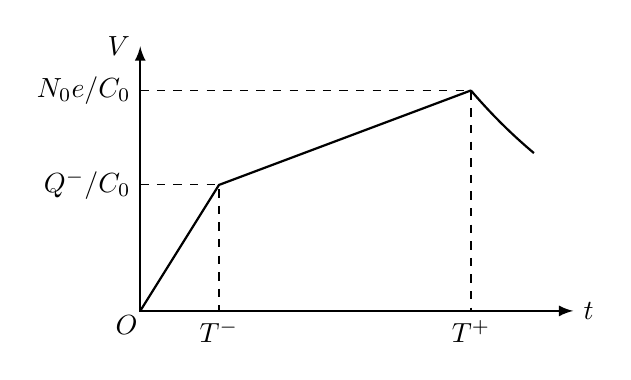
\begin{tikzpicture}[yscale=.8]
    \xOy t{5.5}V{4.2};
    \draw[thick](0, 0)--(1, 2)--(4.2, 3.5);
    \draw[thick, domain=4.2:5]plot(\x, {3.5^((7.2-\x)/3)});
    \draw[dashed](0, 2)node[left]{$Q^-/C_0$}--(1, 2)--(1, 0)node[below]{$T^-$};
    \draw[dashed](0, 3.5)node[left]{$N_0e/C_0$}--(4.2, 3.5)--(4.2, 0)node[below]{$T^+$};
\end{tikzpicture}

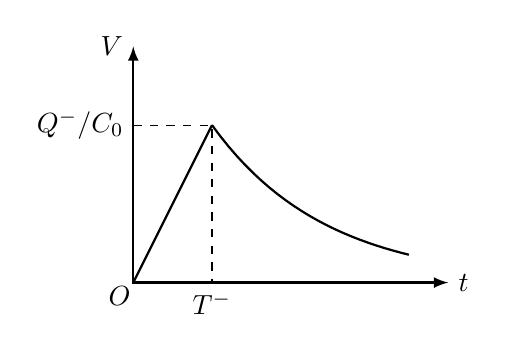
\begin{tikzpicture}
    \xOy t4V3;
    \draw[thick](0, 0)--(1, 2);
    \draw[thick, domain=1:3.5]plot(\x, {2^(2-\x)});
    \draw[dashed](0, 2)node[left]{$Q^-/C_0$}--(1, 2)--(1, 0)node[below]{$T^-$};
\end{tikzpicture}

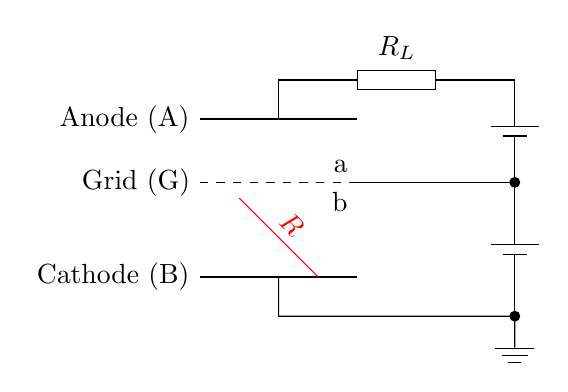
\begin{tikzpicture}[circuit ee IEC]
    \draw [thick] (-4, 2.5) node [left] {Anode (A)} -- (-2, 2.5);
    \draw [thick] (-4, .5) node [left] {Cathode (B)} -- (-2, .5);
    \draw [dashed] (-4, 1.7) node [left] {Grid (G)} -- (-2, 1.7) node [above left] {a} node [below left] {b};
    \draw (-2, 1.7) -- (0, 1.7);
    \draw (-3, .5) to (-3, 0) to (0, 0) to [ground={at end}] (0, -.5);
    \draw (-3, 2.5) to (-3, 3) to [resistor={info={$R_L$}}] (0, 3) to [battery] (0, 1.7) node [contact] {} to [battery] (0, 0) node [contact] {};
    \draw [red] (-3.5, 1.5) -- (-2.5, .5) node [midway, above, sloped] {$R$};
\end{tikzpicture}


\begin{tikzpicture}
    \xOy {V_0}6h4;
    \draw[thick](2, 2)parabola(0, 0);
    \draw[thick](2, 2)--(4, 2.1);
    \draw[thick](4, 2.1)parabola(5, 3)node[above]{正比区};
    \draw[dashed](0, 2)--(2, 2);
    \draw[dashed](0, 1.8)node[left]{90\%}--(1.37, 1.8)--(1.37, 0)node[below]{$V_1$};
    \draw[dashed](4, 2.1)--(4, 0)node[below]{$V_2$};
    \draw[dashed](2.25, 2)--(2.25, 0)node[below]{$V_{\mathrm{work}}$};
    \node[above right]at(0, 3){复合区};
    \node[above]at(2.75, 3){饱和区};
\end{tikzpicture}

\begin{tikzpicture}
    \xOy h6n4;
    \draw[thick, domain=0:1.5]plot(\x, {3*exp(-4*\x*\x)});
    \node[right]at(0, 3){电子学噪声};
    \draw[dashed, domain=.25:1.75]plot(\x, {2*exp(-16*(\x-1)*(\x-1))});
    \node[below]at(1, 0){复合区};
    \draw[thick, domain=-1:1, shift={(3.6, 0)}]plot(\x, {1.2*exp(-6*\x*\x)});
    \draw[thick, domain=-1:1, shift={(4, 0)}]plot(\x, {exp(-4*\x*\x)});
    \draw[thick, domain=-1:1, shift={(4.4, 0)}]plot(\x, {.8*exp(-3*\x*\x)});
    \draw[dashed](3.6, 0)node[below]{$h_1$}--(3.6, 1.5);
    \draw[dashed](4, 0)node[below]{$h_2$}--(4, 1.5);
    \draw[dashed](4.4, 0)node[below]{$h_3$}--(4.4, 1.5);
    \node at(3, -1){(a)};
\end{tikzpicture}
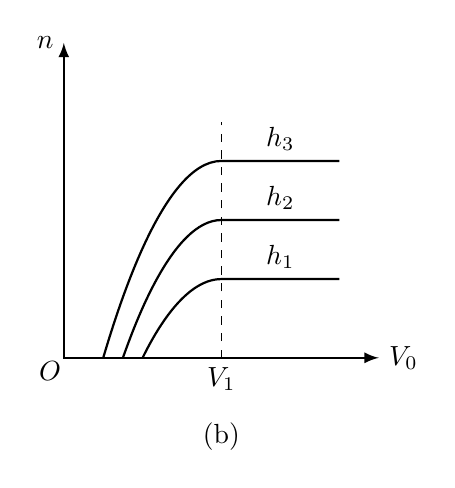
\begin{tikzpicture}
    \xOy {V_0}4n4;
    \draw[dashed](2, 0)node[below]{$V_1$}--(2, 3);
    \draw[thick](3.5, 1)--(2, 1)node[midway, above]{$h_1$}parabola(1, 0);
    \draw[thick](3.5, 1.75)--(2, 1.75)node[midway, above]{$h_2$}parabola(.75, 0);
    \draw[thick](3.5, 2.5)--(2, 2.5)node[midway, above]{$h_3$}parabola(.5, 0);
    \node at(2, -1){(b)};
\end{tikzpicture}

\end{document}